\documentclass[11 pt]{article}

\setlength{\oddsidemargin}{-.45in}
%\setlength{\evensidemargin}{-.5in}
\setlength{\textwidth}{7.25in}
\setlength{\topmargin}{-0.95in}
\setlength{\textheight}{10.2in}

\usepackage{graphics}
\usepackage{latexsym}
\usepackage{amsfonts}
\usepackage{amsmath}
\usepackage{amsthm}
\usepackage{epstopdf}
%\usepackage{multicol}
%\usepackage{wrapfig}
\pagestyle{empty}

\usepackage[T1]{fontenc}
\usepackage{baskervald}
\usepackage[bigdelims,vvarbb]{newtxmath} 

\newcommand{\ds}{\ensuremath{\displaystyle}}
\newcommand{\tr}{\vspace{0.5in}}
\newcommand{\lr}{\vspace{1.0in}}
\newcommand{\mr}{\vspace{2.0in}}
\newcommand{\br}{\vspace{3.0in}}

\newcommand{\ps}{Problem Set~}
\newcommand{\vi}{\ensuremath{\mathbf{i}}}
\newcommand{\vj}{\ensuremath{\mathbf{j}}}
\newcommand{\vk}{\ensuremath{\mathbf{k}}}
\newcommand{\vr}{\ensuremath{\mathbf{r}}}
\newcommand{\vecv}{\ensuremath{\mathbf{v}}}
\newcommand{\vu}{\ensuremath{\mathbf{u}}}
\newcommand{\va}{\ensuremath{\mathbf{a}}}
\newcommand{\vs}{\ensuremath{\mathbf{s}}}
\newcommand{\ve}{\ensuremath{\mathbf{e}}}
\newcommand{\vx}{\ensuremath{\mathbf{x}}}
\newcommand{\vc}{\ensuremath{\mathbf{c}}}
\newcommand{\vb}{\ensuremath{\mathbf{b}}}

\usepackage{hyperref} 
\hypersetup{colorlinks=true, linkcolor=blue,  anchorcolor=blue,  
citecolor=blue, filecolor=blue, menucolor=blue, pagecolor=blue,  
urlcolor=blue,pdftitle={MTH 202 Checkpoint}}

\usepackage{framed}

\newcommand{\bdr}{\ensuremath{\mathbb{R}}}

\newcommand{\be}{\begin{enumerate}}
\newcommand{\ee}{\end{enumerate}}

\newcommand{\bi}{\begin{itemize}}  
\newcommand{\ei}{\end{itemize}}

%\renewcommand{\baselinestretch}{1.5}


\begin{document}
 \hfill Boelkins \\
 
\begin{center}
Math 202-06 \\
{\bf Checkpoint 7}
\end{center}


\noindent {\bf Directions:}

\begin{itemize}
	
	\item {\bf Desmos.} You may use \href{https://www.desmos.com/calculator}{\emph{Desmos}} for computations and graphing, just like we do during class.  Any work done in \emph{Desmos} must be summarized and briefly explained in writing on your paper.  
	
	\item {\bf Resources.} During each checkpoint, you may access your own 1 page of study notes, plus \emph{Desmos}; no other uses of your computer or tablet are permitted unless specified directly.  No collaboration with other human beings or other internet resources are allowed.
	
%	\emph{Note well: if you collaborate with someone else, it is often obvious that collaboration has occurred.  Please do not put your academic standing at risk by doing this.}
	
	\item {\bf Competence.} Each week, your goal is to demonstrate competence on as many of the included learning targets as you can.  Each question will be marked either ``Y'' or ``NY'': Y for ``yes'', NY for ``not yet''.  Every learning target will appear on three different checkpoints, so you'll have multiple attempts to demonstrate your understanding.  ``Competence'' is defined as work that demonstrates clear and complete understanding of the relevant concepts in the learning target. While the work may include a minor error, or one or two minor steps may not be well explained, otherwise the work is complete, correct, and convincing, including the proper use of notation, and appropriate explanation of meaning that uses correct terminology.  (On rare occasions, you might get a ``NY*''; such a mark means you are close to competence and that you have the option to have a short conversation with me prior to the next Checkpoint and attempt to demonstrate ``Y''-level understanding through the conversation aloud.)	
\end{itemize}

\noindent \hrulefill \\

\noindent {\bf Learning Targets:} For Checkpoint \#7, there are three learning targets being assessed: 

\begin{quote}
{\bf LT 6}: I can use definite integrals to find the area between two curves and the volume of a solid of revolution. (Sections 6.1 and 6.2)
\end{quote}

\begin{quote}
{\bf LT 7}: I can use definite integrals to find the mass and center of mass of an object.
\end{quote}

\begin{quote}
{\bf LT 8}: I can use definite integrals to represent key quantities in applications such as the work done by a varying force or the pressure that water exerts against a dam. (Section 6.4)
\end{quote}

\noindent \hrulefill \\

\vfill \hfill {\bf OVER} 

\pagebreak

\noindent Name: \\ 

\noindent To demonstrate competence on Learning Target \#$n$, you need to correctly respond to all or nearly all of the prompts in question \#$n$.  

\begin{enumerate}


%{\bf LT 6}: I can use definite integrals to find the area between two curves and the volume of a solid of revolution. (Sections 6.1 and 6.2)


\item[6.] For each of the following prompts, {\bf set up, but do not evaluate, a single definite integral that gives the area or volume of each region described}.  Your processes are even more
important than your final answers here, so show all of your work in a clear and logical order. \emph{For each, include a careful, labeled plot, a representative slice, the area/volume of that representative slice, and make
sure your final answer is clearly indicated (for example by circling it).}
	
	
	\be
		\item The exact area of the finite region bounded by $x = -(y-2)^2$ and $y = x + 6$. \\
		
		\scalebox{0.27}{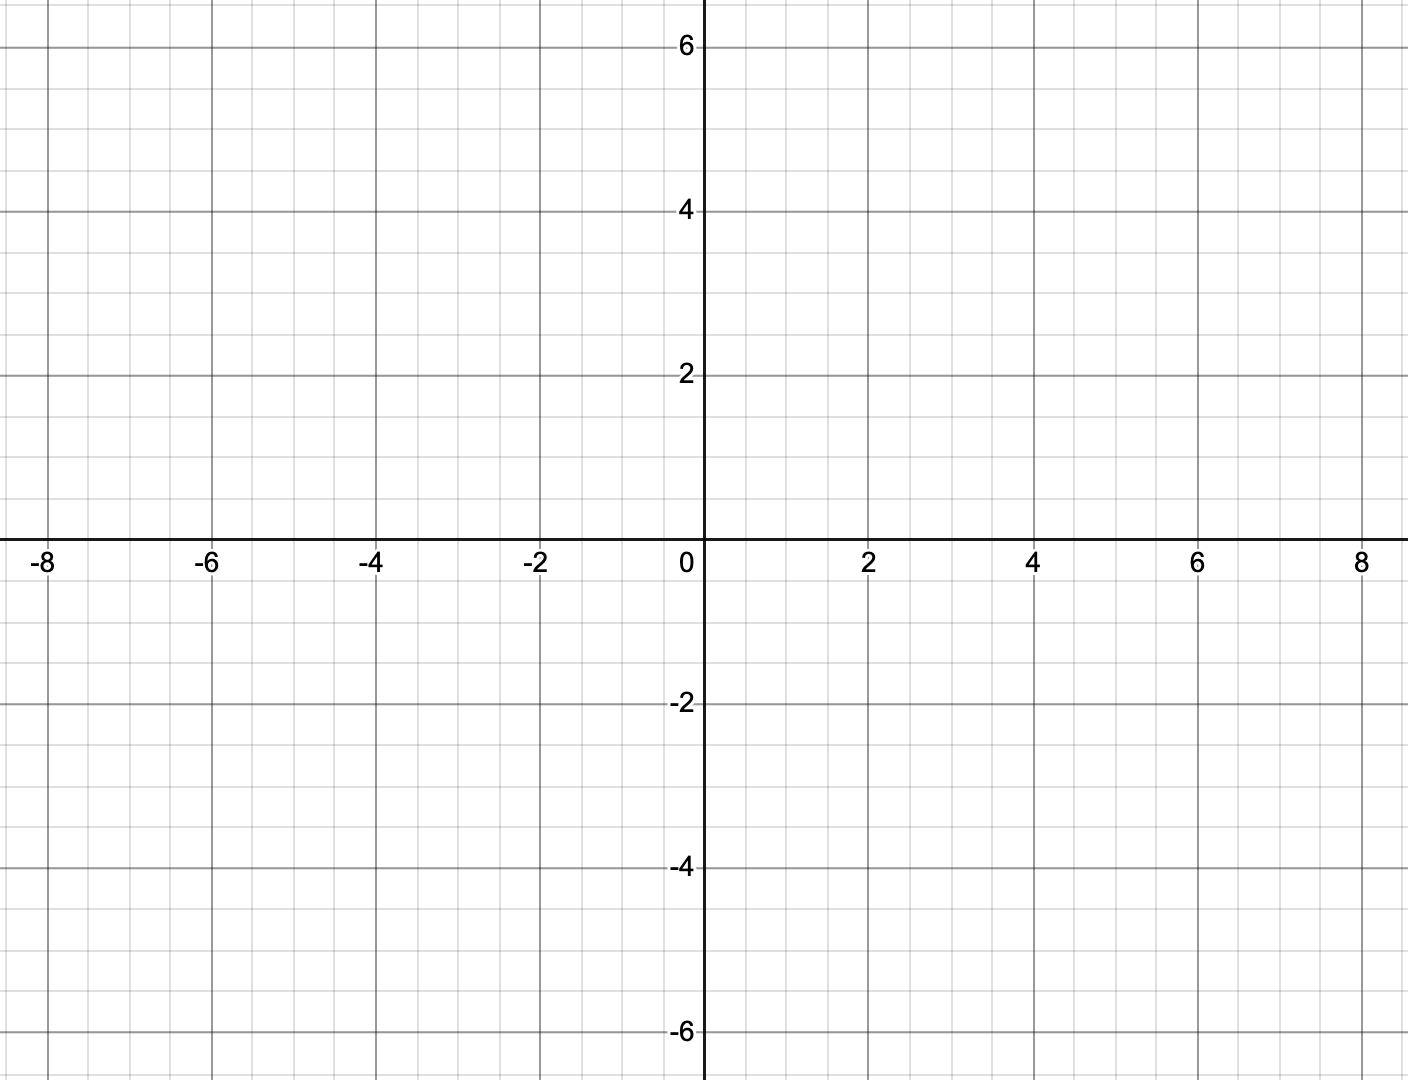
\includegraphics{images/CP-5-blank-grid-LT6.png}} \\
	 	
		\item The exact volume that results from taking the finite region bounded by $y = \frac{1}{2}(x-3)^2+2$ and $x = 5 - y$ and revolving that region about the $x$-axis. \\
		
		\scalebox{0.27}{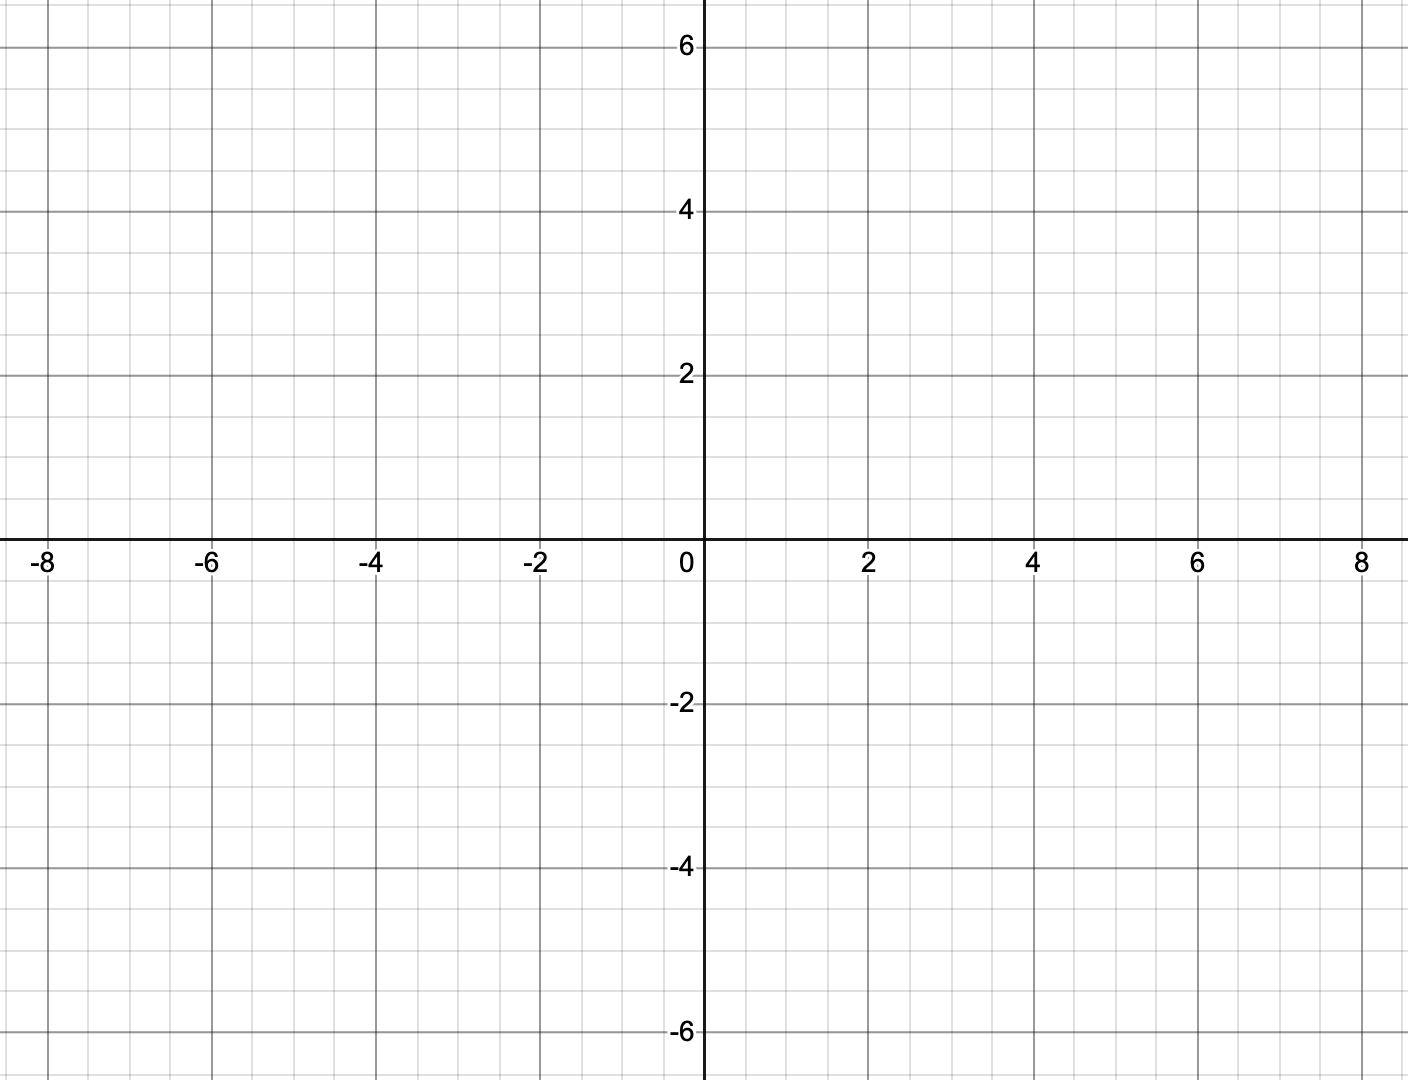
\includegraphics{images/CP-5-blank-grid-LT6.png}} \\
	 	
		\item The exact volume that results from taking the finite region bounded by $y = \frac{1}{2}(x-3)^2+2$ and $x = 5 - y$  and revolving that region about the $y$-axis. \\
		
		\scalebox{0.27}{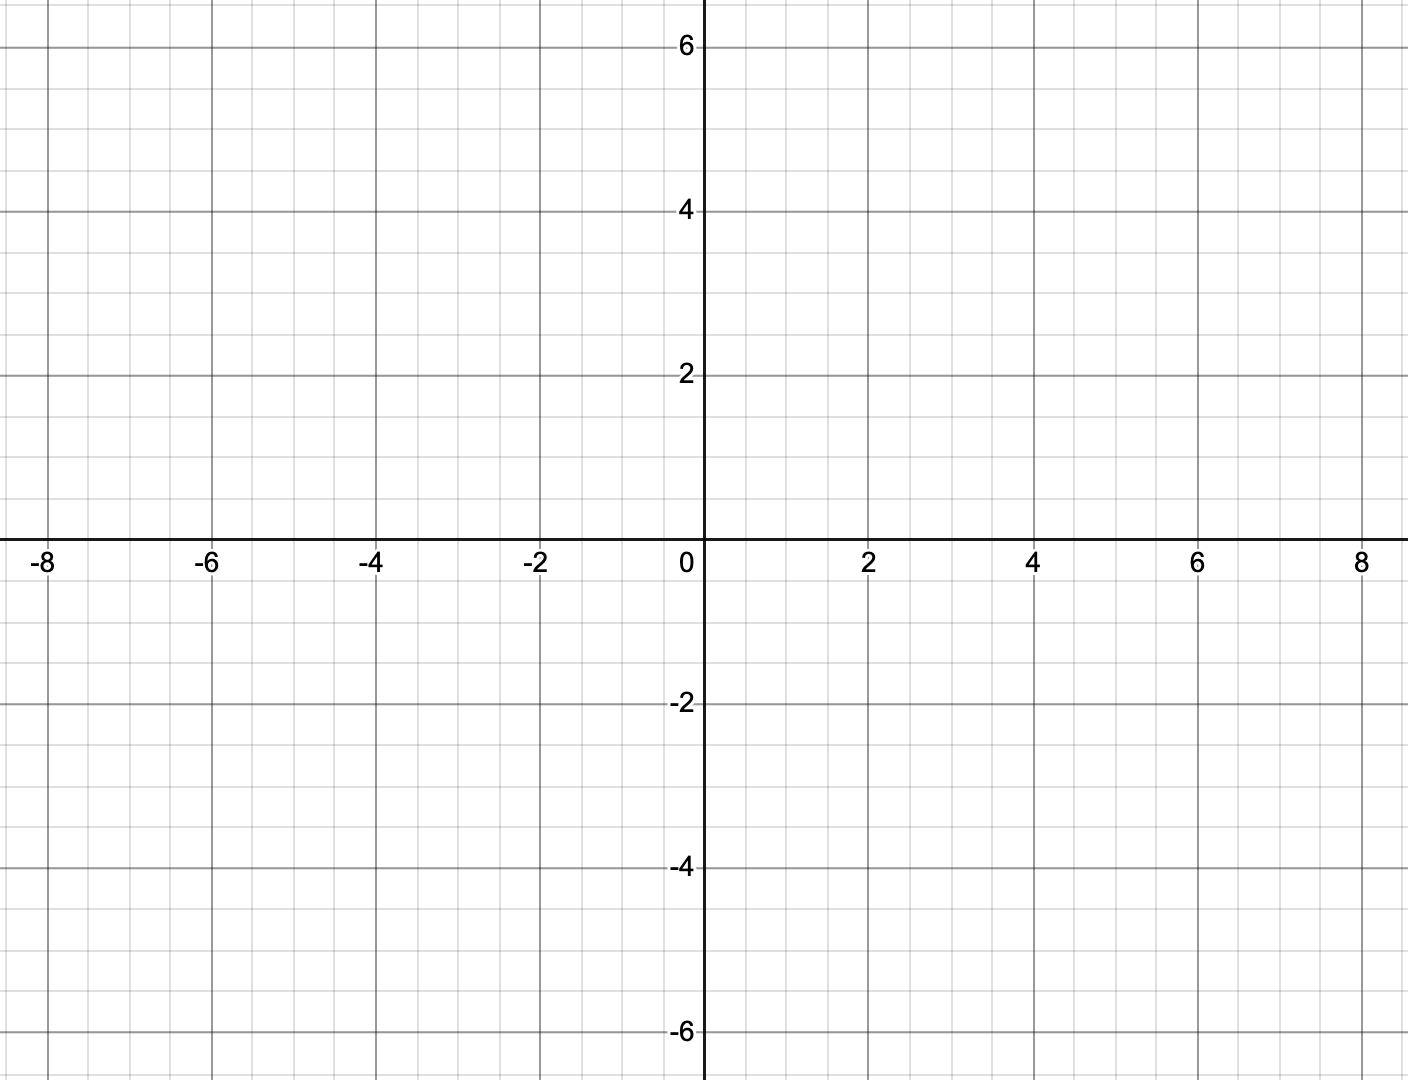
\includegraphics{images/CP-5-blank-grid-LT6.png}} \\		
	\ee


\pagebreak

\noindent Name: \\ 

%{\bf LT 7}: I can use definite integrals to find the mass and center of mass of an object.

\item[7.]  Let a thin rod with constant cross-sectional area of $1$ cm$^2$ be given.  Assume the rod is 6 cm long and is situated so that its left end lies at $x = 0$ on the horizontal axis.  Suppose that the rod's density is distributed along the rod by the function $\rho(x) = 2e^{-(x-4)^2}$, measured in grams per cm.

	\be
		\item From the graph of $\rho(x)$ (without doing any computations), do you expect the rod's center of mass, $\overline{x}$, to lie at $x = 3$, left of $x = 3$, or right of $x = 3$?  Why?
		
		\tr \tr
		
		\item Find the mass $M$ and center of mass $\overline{x}$ by stating appropriate definite integrals and evaluating them using technology.  Clearly identify your results.
		
		\mr \tr
		
		\item From the graph of $\rho(x)$ (without doing any computations), how would the rod's mass and center of mass change (if at all) if the density function was instead $\rho(x) = 2e^{-(x-2)^2}$?  Write a sentence to discuss.
		
		\tr \tr
		
		\item Returning to the original density function function $\rho(x) = 2e^{-(x-4)^2}$ for the bar of length 6 cm, estimate the value of $a$ for which 90\% of the mass of the bar lies to the left of $a$.  Show a clear summary of your work and thinking. 
	\ee	

\pagebreak

\noindent Name: \\ 

% {\bf LT 8}: I can use definite integrals to represent key quantities in applications such as the work done by a varying force or the pressure that water exerts against a dam. (Section 6.4)

\item[8.] Consider a trough with a trapezoidal end as pictured below.


Assume the trough is 14 feet wide along its top, 12 feet wide along its bottom, 7 feet deep, 20 feet long, and that it is full of water to a depth of 6 feet.   As usual, the weight density of water is 62.4 pounds per cubic foot.

\be
	\item \emph{Determine the total amount of work that would be required to empty the top 3 feet of water from the tank and pump the water to a truck whose tank is 5 feet above the top of the tank}.  In your response, clearly sketch and label the relevant slice(s) and show the steps and thinking that are involved in determining the definite integral that answers the question.  Conclude your work with the appropriate definite integral clearly and evaluate it using technology to determine the total work to achieve the task noted above.  Include units on your result.
	
\hfill \scalebox{0.5}{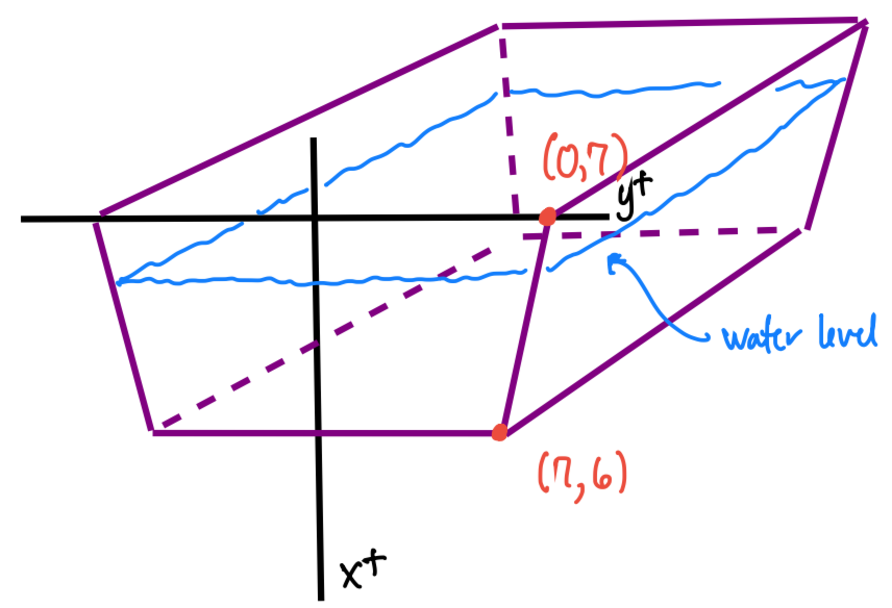
\includegraphics{images/LT8-trough}}

\lr
	
	\item Now suppose that the tank is back in its initial state: full of water to a depth of 6 feet.  \emph{Determine the total amount of hydrostatic force on one end of the trough}.  In your response, clearly sketch and label the relevant slice(s) and show the steps and thinking that are involved in determining the definite integral that answers the question.  Conclude your work with the appropriate definite integral clearly and evaluate it using technology to determine the total work to achieve the task noted above.  Include units on your result.

\ee  

\hfill \scalebox{0.5}{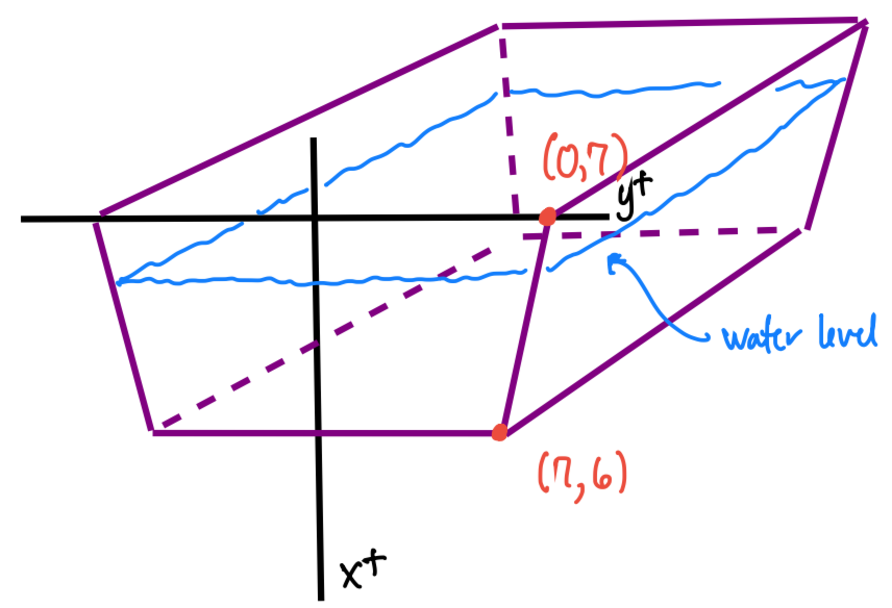
\includegraphics{images/LT8-trough}}

\lr
	
	
\end{enumerate}



\end{document}
